% Comparaison entre gammes de puissance
\section{Comparer les gammes de puissance}
\label{sec:comparaison}

\subsection{Débit et puissance rapportés}

La figure~\ref{fig:fps-power} place les 79 lignes de \texttt{benchmarks.csv} qui ont à la
fois un débit et une puissance, sur 324. Les points pleins ont une puissance mesurée (puce
ou carte) ; les points creux, une puissance estimée ou de \gl{portee}{portée} non décrite.

\begin{figure}[!htbp]
\centering
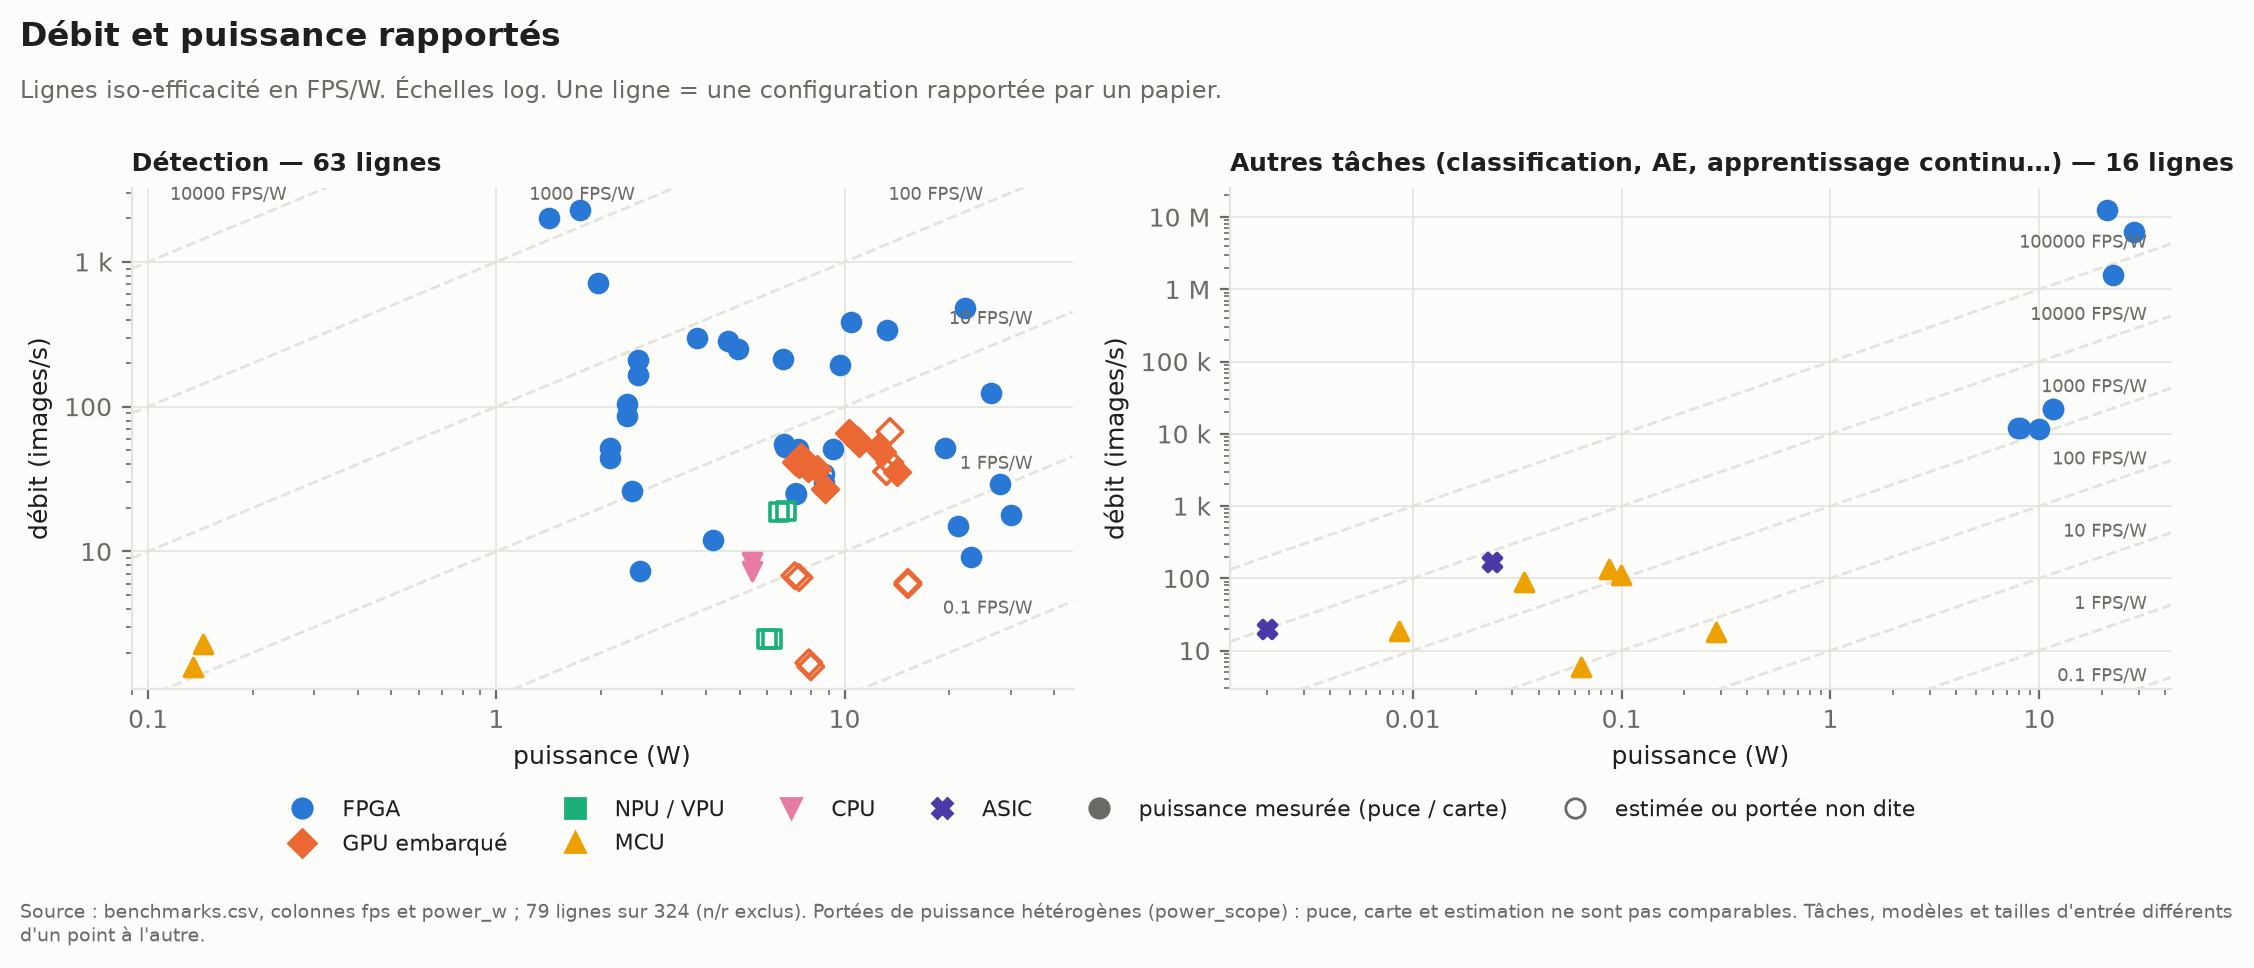
\includegraphics[width=\textwidth]{../../figures/bench_fps_power.png}
\caption{Débit et puissance rapportés, en échelles logarithmiques ; droites pointillées
d'iso-efficacité en FPS/W. Figure générée par \texttt{bin/pdb plot} à partir de
\texttt{benchmarks.csv} (28/09/2026).}
\label{fig:fps-power}
\end{figure}

Pour la détection (panneau de gauche), la figure montre trois groupes. Les deux points
\gl{MCU}{MCU} (SSD-MobileNetV2 sur GAP8) sont vers 0,14\,W et 2\,\gl{FPS}{FPS}. Les \gl{GPU}{GPU} embarqués (Jetson) se
regroupent entre 7 et 15\,W pour quelques dizaines d'images par seconde. Les \gl{FPGA}{FPGA}
s'étalent sur trois ordres de grandeur de débit, de 1,4 à 30\,W ; les points au-dessus de
1\,000\,FPS sont les réseaux minuscules du \gl{DAC-SDC}{DAC-SDC}, mesurés sans chargement d'images. Ce
que la figure ne permet pas : conclure qu'une famille est plus efficace qu'une autre.
Aucun couple de points ne partage à la fois le modèle, la résolution, la précision
numérique et la méthode de mesure \deduit.

\subsection{Les rares comparaisons à modèle égal}

\begin{table}[!htbp]
\centering\footnotesize
\caption{Comparaisons du corpus où un même réseau est mesuré sur plusieurs familles de
plateformes.}
\label{tab:meme-modele}
\begin{tabularx}{\textwidth}{@{}P{3.0cm}P{2.4cm}LP{3.2cm}@{}}
\toprule
Travail & Modèle & Résultat & Réserve \\
\midrule
SkyNet \citep{arxiv-1909.09709-skynet-hardware-efficient-method-object}\pp & SkyNet,
  DAC-SDC & TX2 : 67,3\,FPS, 13,5\,W ; Ultra96 : 25,1\,FPS, 7,3\,W \src{Tables~5--6} &
  portée non décrite ; \gl{lot}{lot de} 4 sur FPGA \\
SATAY \citep{2023-montgomerie-corcoran-satay-streaming-architecture-toolflow-accelerating} &
  YOLOv5n 640 & ZCU104 : 317\,mJ/image ; TX2 : 277\,mJ \src{Table~IV}\med & portée non
  décrite ; runtime du TX2 \nr \\
\citet{2025-elhence-fpga-accelerated-yolox-enhanced-attention} & LCAM-YOLOX & KV260 : 195\,FPS ;
  Jetson Nano : 65\,FPS ; STM32H7A3 : 15\,FPS \src{§V-D}\med & précision et puissance \nr{}
  hors FPGA ; chiffre MCU invraisemblable \\
TinyissimoYOLO \citep{arxiv-2306.00001-tinyissimoyolo-quantized-low-memory-footprint} & réseau
  88$\times$88 & MAX78000 : 5,5\,ms, 196\,µJ ; Apollo4b : 6,1\,mJ \src{§III}\med & MCU
  seulement \\
\citet{arxiv-2502.15737-performance-analysis-you-only-look} & YOLOv8n \gl{INT8}{INT8} & Orin NX :
  65,8\,FPS, 10,3\,W ; Orin Nano : 44,9\,FPS, 7,5\,W \src{Table~4} & Jetson seulement ;
  \gl{telemetrie}{télémétrie} ; jeu privé facile \\
\citet{arxiv-2409.16808-comprehensive-evaluation-deep-learning-object}\pp & YOLOv8n & Orin
  Nano : 16\,ms ; RPi~5 + Hailo-8 : 76\,ms ; \gl{mAP}{mAP} \gl{COCO}{COCO} 31--32 \src{§IV}\med & précision
  numérique \nr ; pas de FPGA \\
\citet{2022-feng-benchmark-analysis-yolo-performance-edge} & YOLOv3-tiny & Xavier NX :
  41,1\,FPS ; RPi + NCS2 : 18,8 ; Nano : 6,8 \src{Table~3} & pas de mAP ; sans TensorRT \\
\bottomrule
\end{tabularx}
\end{table}

Le tableau~\ref{tab:meme-modele} montre qu'aucun article ne mesure le même détecteur sur
les trois gammes (nano, FPGA, Jetson) avec la même portée de puissance. Les comparaisons
FPGA--Jetson existantes utilisent des Jetson de 2017 (TX2) ou des modèles minuscules ; la
seule qui ajoute un MCU (Elhence et al.) n'est pas crédible sur ce point. Les baselines
Jetson récentes (Orin, TensorRT INT8) existent dans le corpus
\citep{arxiv-2502.15737-performance-analysis-you-only-look}, mais sans FPGA en face.

\subsection{Ordres de grandeur par gamme}

Faute de comparaison directe, le corpus donne des ordres de grandeur, à ne lire que
comme tels :
\begin{itemize}
  \item \textbf{nano} : de 4 à 41\,\gl{MAC}{MMAC} par image pour la navigation, 534\,MMAC pour le
    seul détecteur déployé (SSD-MbV2, 1,6\,FPS) ; de 34 à 284\,mW ; 0,4\,mJ par image pour
    la pose humaine \citep[§V-B]{arxiv-2103.10873-fully-onboard-ai-powered-human}\pp ;
  \item \textbf{FPGA} : de 2,5\,W (Zynq-7020, carte) à 10\,W (KV260, carte) et 30\,W (ZCU104,
    à la prise), pour des \gl{YOLO}{YOLO} réduits à quelques centaines de FPS d'accélérateur, et
    quelques dizaines de \gl{bout}{bout en bout} ;
  \item \textbf{Jetson} : de 7 à 15\,W de télémétrie pour YOLOv8n et YOLOv8s en INT8
    (45 à 66\,FPS), 40\,ms pour les réseaux de vol agile sur TX2, de 23 à 35\,FPS pour les
    trackers et GLAD sur Xavier.
\end{itemize}
L'écart entre gammes est de l'ordre de trois ordres de grandeur en puissance, mais la
tâche change aussi : navigation en 200$\times$200 en niveaux de gris d'un côté, détection
en 640$\times$640 de l'autre \deduit.

\subsection{Couverture du corpus}

La figure~\ref{fig:gaps-map} croise la famille de plateforme des mesures et l'axe des
articles. Elle confirme les déséquilibres décrits dans ce document : la détection drone
est surtout mesurée sur GPU de bureau (17 articles), le contre-drone aussi (9 articles),
aucune mesure FPGA ne concerne un nano-drone et aucune mesure du corpus ne porte sur la
fiabilité. Un zéro signifie \enquote{absent de la base}, pas \enquote{absent de la
littérature}.

\begin{figure}[!htbp]
\centering
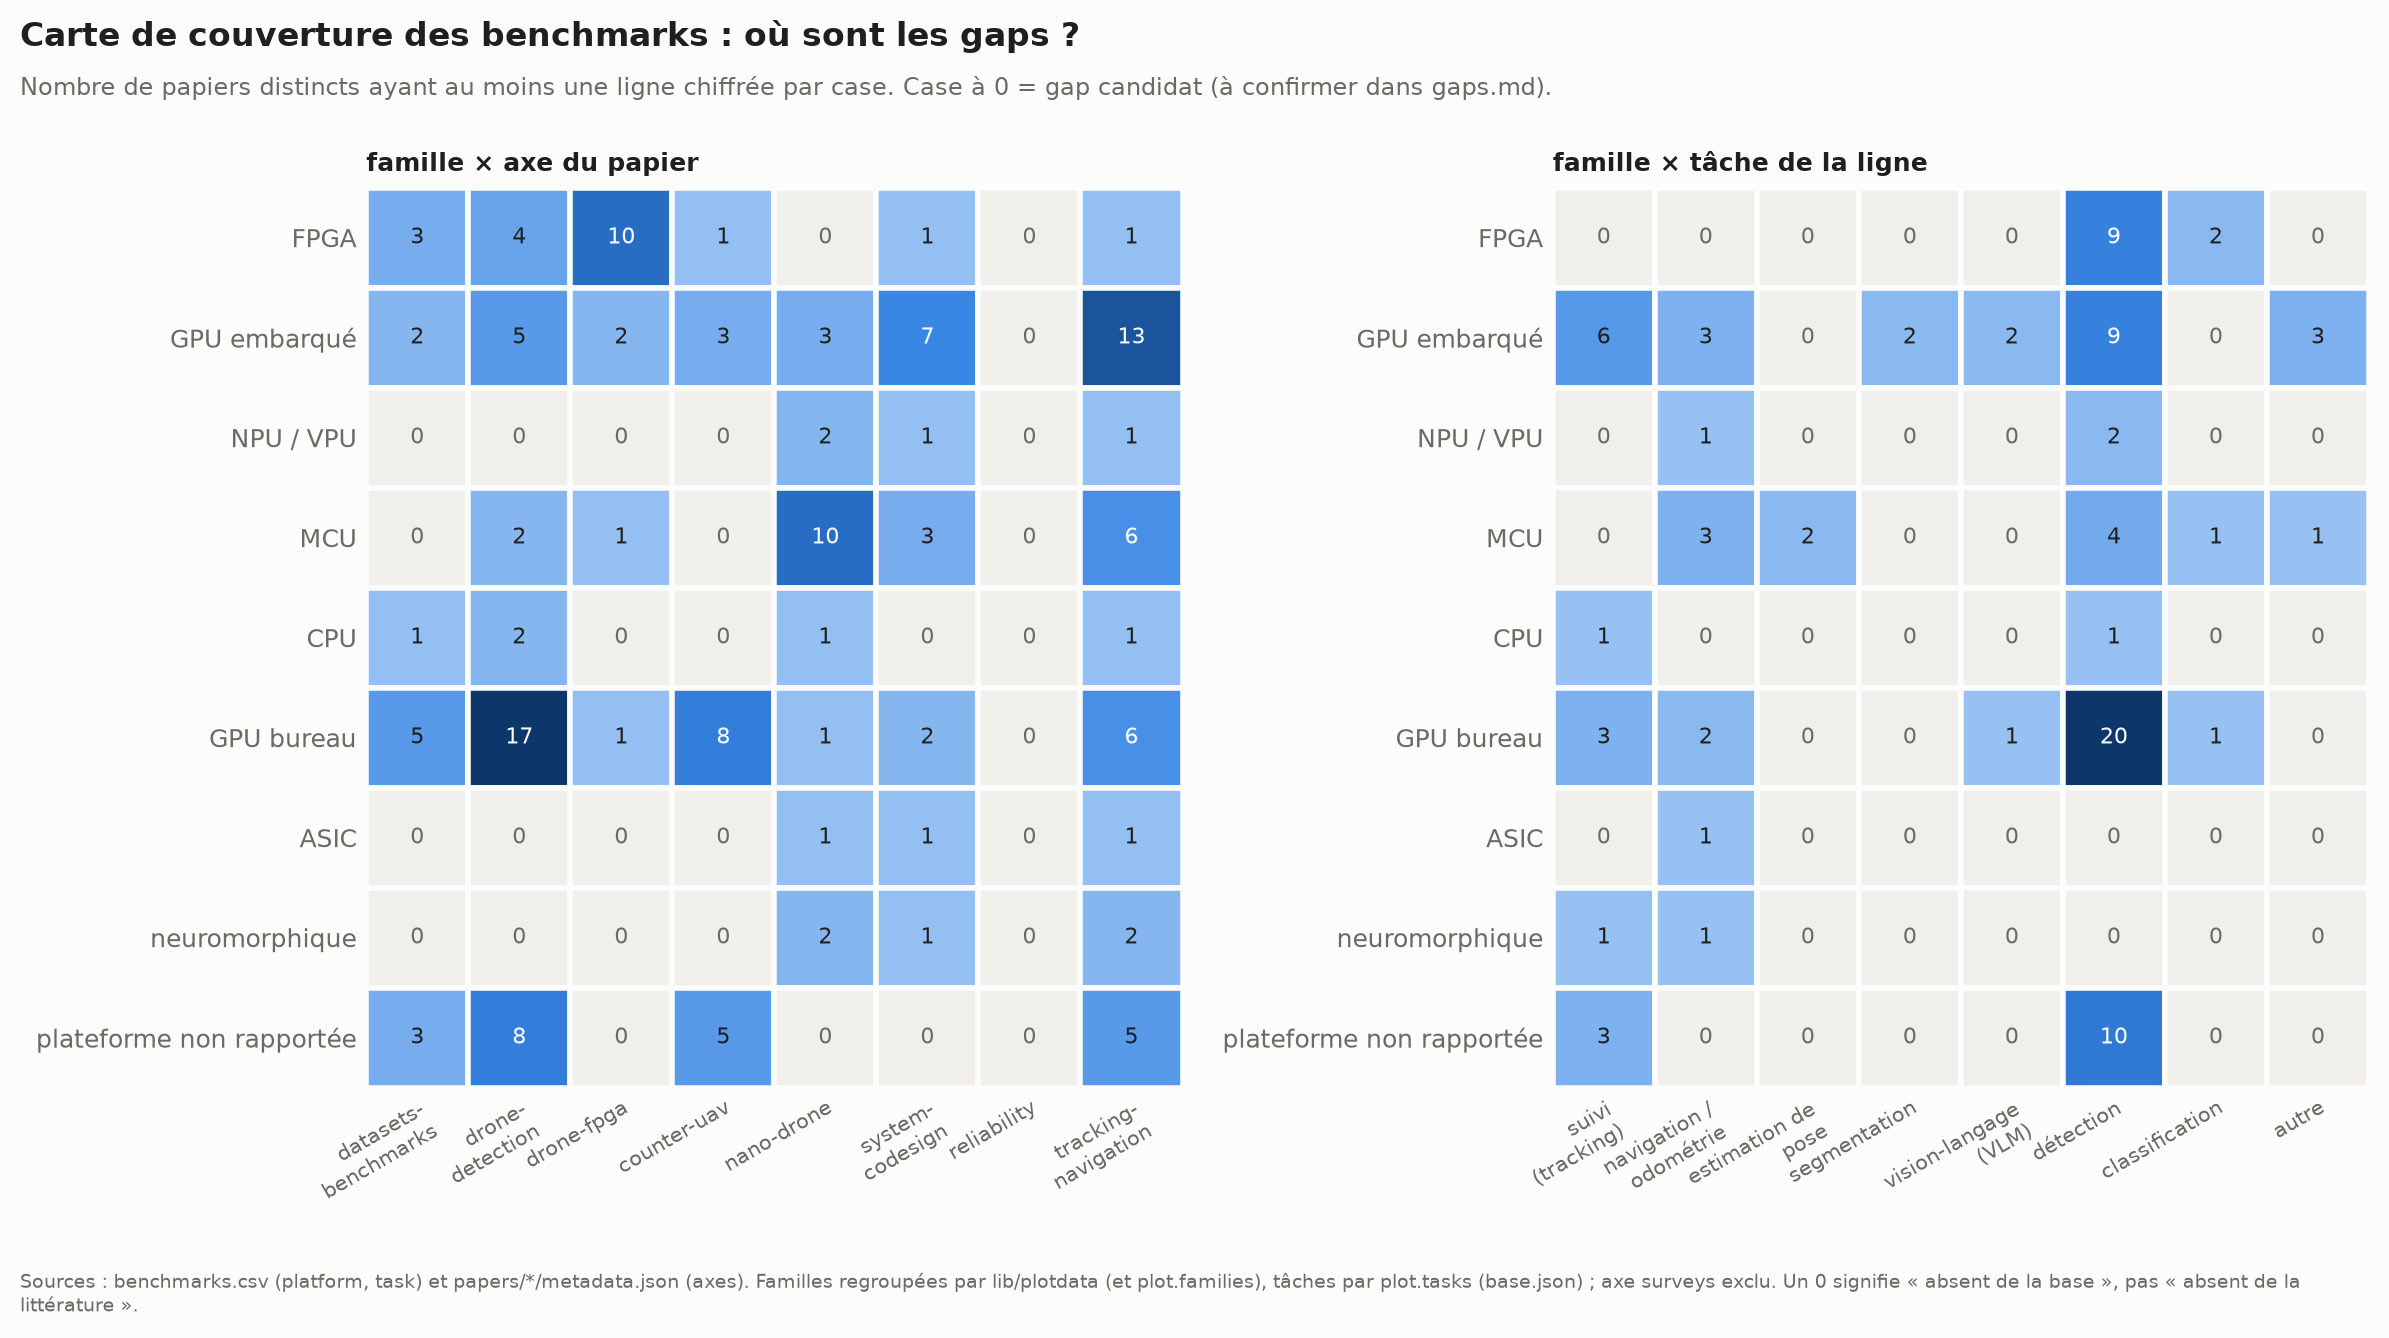
\includegraphics[width=\textwidth]{../../figures/corpus_gaps.png}
\caption{Nombre d'articles ayant au moins une ligne chiffrée, par famille de plateforme et
par axe (gauche) ou tâche (droite). Figure générée par \texttt{bin/pdb plot} (28/09/2026).}
\label{fig:gaps-map}
\end{figure}
